\section{El problema del viajante de comercio}

\begin{frame}{Problema}
Hallar el recorrido con distancia mínima en un conjunto de
ciudades que pase por todas las ciudades y regrese al punto inicial.

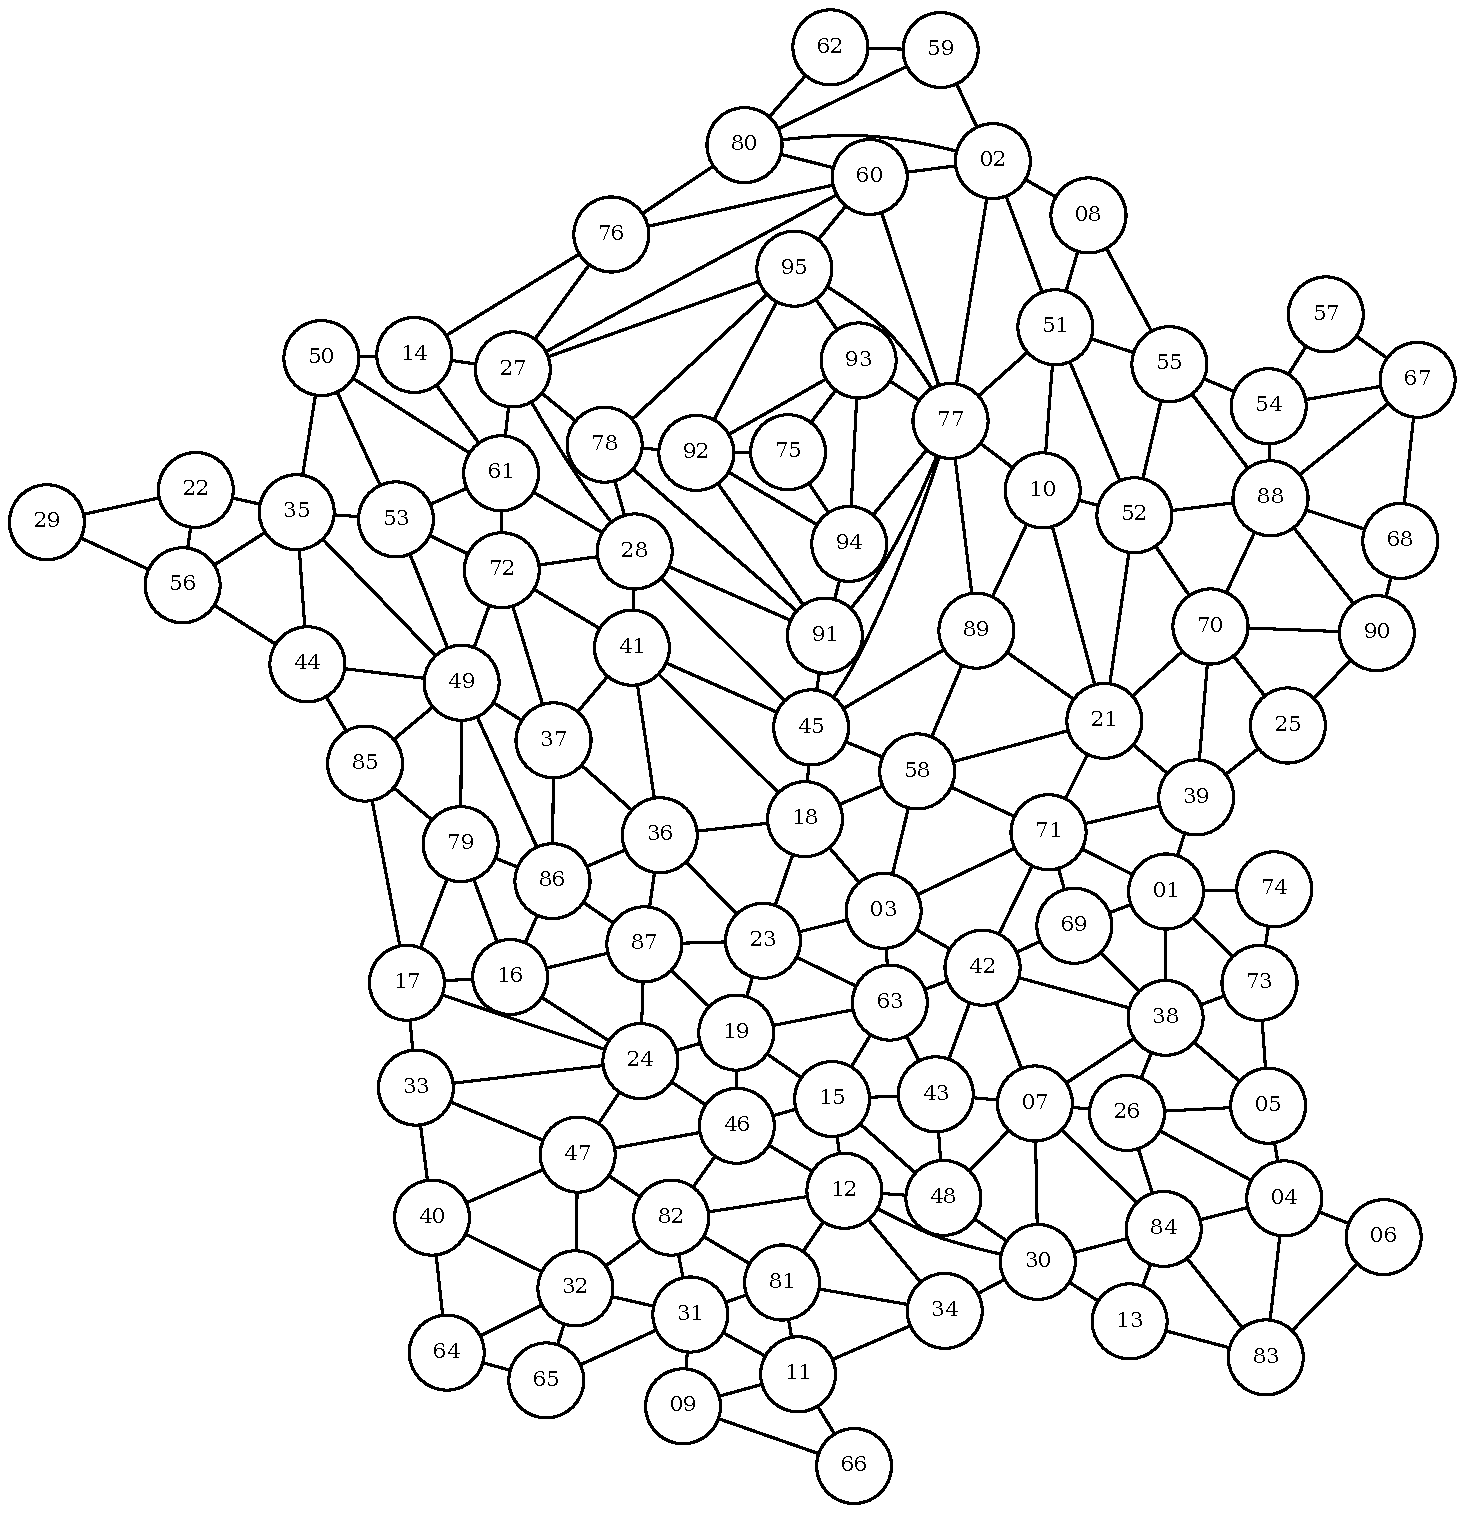
\includegraphics[width=.5\textwidth]{img/Francia} \centering
\end{frame}

\begin{frame}{Algoritmos}
\begin{description}
 \item[Entrada:] Ficheros con ciudades indicadas como puntos en el plano según sus
 coordenadas.
 \item[Salida:] \texttt{vector<int>} con el orden en el que se recorren las ciudades.
\end{description}
\end{frame}

% TODO: todo lo posterior

\begin{frame}{\texttt{Grafo}}
Un grafo consta de:

\begin{itemize}
  \item Una \textbf{cantidad de nodos}: \texttt{nodos}.
  \item Una \textbf{matriz de pesos}: \texttt{lados}.
\end{itemize}
\end{frame}

\subsection{Ramificación y acotación}

\begin{frame}{Algoritmo general}
  Iniciamos:
  \begin{itemize}
    \item La cola con la solución parcial \texttt{[0]}
    \item La mejor solución con un algoritmo \textit{greedy} (vecino más cercano)
  \end{itemize}
\end{frame}

\begin{frame}{Algoritmo general}
  Mientras la cola no esté vacía, coge el primer elemento:
  \begin{itemize}
    \item Si \textbf{puede formarse una solución completa}, comprueba si es mejor que la mejor encontrada. En tal caso actualizala y borra los nodos con peor cota.
    \item En \textbf{otro caso}, para cada ciudad no visitada forma una nueva solución parcial. Añádela a la cola si su cota es mejor que la mejor solución.
  \end{itemize}
\end{frame}

\subsubsection{Cotas}

\begin{frame}{Cota del mínimo}
  Calcular la longitud del recorrido inicial y suma la menor distancia de cada ciudad no incluida en la solución parcial con sus relacionadas.
\end{frame}

\begin{frame}{Arbol generador}
  Calcular la longitud del recorrido que se lleva hasta ese momento, y suma la longitud del árbol generador minimal de los nodos que faltan junto al último nodo del camino. Además, se suma la mínima longitud del primer nodo a otro más.

  %% Aquí pintad en pizarra que si no, no lo entiende ni dios, y es una tontería
\end{frame}

\subsection{Vuelta atrás}

%% TODO: (Iñaki) Descripción del algoritmo de backtracking

\subsection{Comparativa de los algoritmos}

\begin{frame}{Ejemplo con 5 nodos}
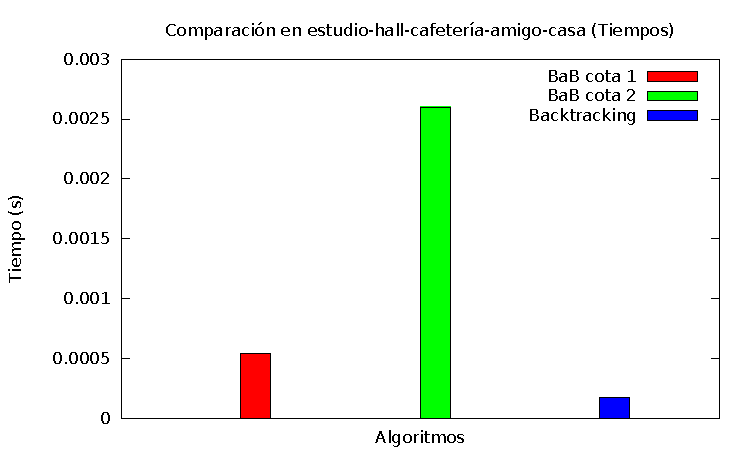
\includegraphics[width=\textwidth]{img/barras_e-h-c-a-c5_t}
\end{frame}

\begin{frame}{Ejemplo con 10 nodos}
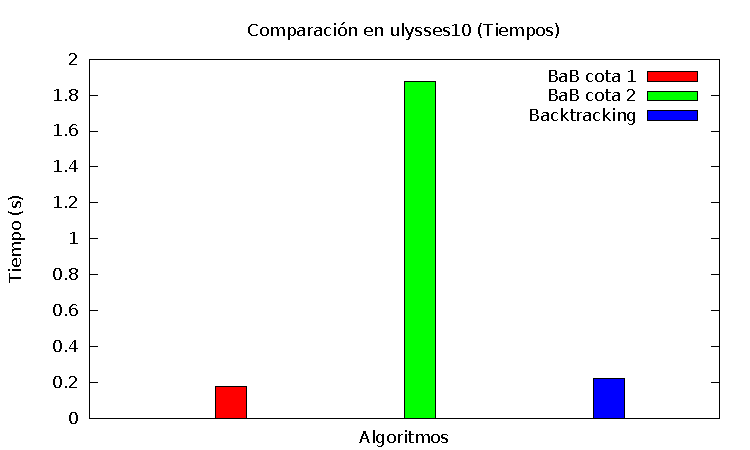
\includegraphics[width=\textwidth]{img/barras_ulysses10_t}
\end{frame}

\begin{frame}{Ejemplo con 12 nodos}
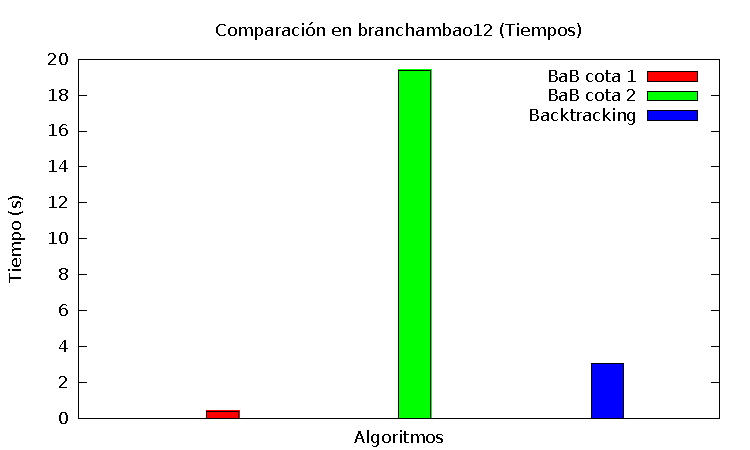
\includegraphics[width=\textwidth]{img/barras_branchambao12_t}
\end{frame}

%%% TODO (Iñaki)
% Gráficas que comparen entre los 3 algoritmos:
% - Número de nodos expandidos
% - Tamaño máximo de la cola con prioridad
% - Número de veces que se realiza la poda
%%%
